\section{Installer des paquets}
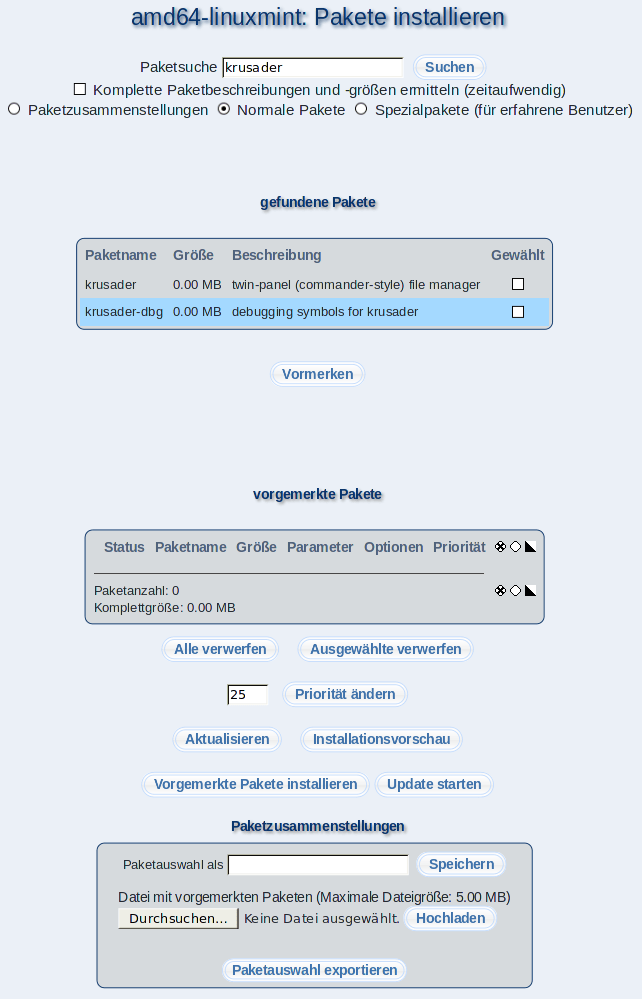
\includegraphics[scale=0.4]{/mdk/doc/manual/screenshots/fr/install_packages.png} \\
\subsection{Notez}
m23 distingue entre trois types de paquet diff�rents:\\
\begin{itemize}
\item \textbf{Combinaisons de paquets:} Ce sont des combinaisons de paquets diff�rents. Vous pouvez empaqueter une quantit� d'applications dans une combinaison de paquets et simplifier l'installation de paquets de programmes identiques sur plusieurs ordinateurs �norm�ment.\\
\item \textbf{Paquets normaux:} Ce sont des paquets de programmes normaux. En g�n�ral, il s'agit des programmes isol�s.\\
\item \textbf{Paquets sp�ciaux (pour utilisateurs exp�riment�s):} Ils contiennent des paquets qui ex�cutent des travaux sp�ciaux comme formater etc., qui devraient �tre utilis�s seulement par des utilisateurs exp�riment�s.\\
\end{itemize}
\subsection{Installer des paquets:}
\begin{enumerate}
\item Choisissez \textit{$\ll$Combinaisons de paquets$\gg$}, \textit{$\ll$Paquets normaux$\gg$} ou \textit{$\ll$Paquets sp�ciaux (pour utilisateurs exp�riment�s)$\gg$}.\\
\item Entrez le mot de recherche pour votre paquet dans le champ de saisie $\ll$Recherche des paquets$\gg$ ou laissez vide le champs si vous voulez laisser chercher tous les paquets d'un type. A cause du grand nombre, cette option n'est pas possible entre les paquets normaux - ici, c'est obligatoire d'entrer un mot de cl\'e.\\
\item Sous \textit{$\ll$Paquets trouv�s$\gg$}, vous voyez tous les paquets qui correspondent \`a vos crit\`eres de recherche.\\
\item Cliquez sur la case \`a cocher derri\`ere les paquets souhait\'es.\\
\item Notez les paquets pour l'installation en cliquant sur \textit{$\ll$Noter$\gg$}.\\
\item R\'ep\'etez les \'etapes 1-5 sur vos besoins.\\
\end{enumerate}
Maintenant, vous avez not\'e des paquets pour l'installation.  Un crochet vert indique que ce paquet est \`a installer, une croix rouge indique que c'est \`a effacer du client. Vous pouvez effacer la liste de ces paquets en cliquant sur \textit{$\ll$Annuler tous$\gg$} ou s\'electionner des paquets et les effacer apr\`es par un clic sur \textit{$\ll$Annuler la selection$\gg$}.\\
Affirmez votre choix en cliquant sur \textit{$\ll$Installer les paquets not�s$\gg$}.\\
\subsection{Pr\'evision de l'installation}
Avant l'installation v\'eritable, vous pouvez voir les cons\'equences de l'installation pour le poste client. De cette fa\c{c}on, vous pouvez voir auparavant quels paquets additionels seront install\'es et s'il y aura des probl\`emes durant l'installation. Pour la pr\'evision, cliquez sur \textit{$\ll$Pr�vision de l'installation$\gg$} apr\`es que vous ayez choisi les paquets. Puis, vous verrez un protocole de la pr\'evision de l'installation.\\
Une pr\'evision est seulement possible si vous avez choisi un poste client singulier et pas de groupe.\\
\subsection{Notez: Combinaisons de paquets}
Si vous cliquez sur \textit{$\ll$Combinaisons de paquets$\gg$}, vous pouvez d�cider si les paquets doivent �tre install�s ou d�sinstall�s du poste client. En plus, vous pouvez garder les actions enregistr�es dans la combinaison de paquets. Ceci vous permet d'utiliser des travaux d'installation et de d�sinstallation dans une combinaison singuli�re. Pour cela, choisissez l'action souhait�e de la liste.\\
\subsection{CONSEIL:}
Si vous voulez enregistrer votre choix de paquets pour pouvoir l'utiliser plus tard, entrez un nom pour votre combinaison de paquets apr�s \textit{$\ll$Nom de la combinaison de paquets$\gg$}et cliquez sur \textit{$\ll$Enregistrer$\gg$}. Cette combinaison sera � votre disposition d�s ce moment-l� dans les \textit{$\ll$Combinaisons de paquets$\gg$}.\\
